\section{Utilisation de \beagle et expériences}
\label{sec:experiences}

\subsection{Présentation de \beagle}
\beagle est un prouveur du premier ordre avec arithmétique très récent,
prenant en entrée le format \tff. Des résultats expérimentaux (sur une
version plus ancienne) ainsi que la théorie détaillée de \beagle peuvent être trouvés dans~\cite{DBLP:conf/cade/BaumgartnerW13}.


\subsection{La tactique \beagletac}
\label{sec:experiences:beagletac}

Voici un diagramme représentant l'ensemble des étapes de \beagletac:

\begin{tikzpicture}[node distance = 2cm, auto]
  % Place nodes
  \node [cloud] (problem) {problème};
  \node [block, right of=problem,  node distance=3cm] (HOL1) 
  {traduction};
  \node [block, right of=HOL1,  node distance=3cm] (HOLTFF1) 
  {impression};
  \node [block, right of=HOLTFF1, node distance=3cm] (TFF1) 
  {fichier problème};
  \node [block, right of=TFF1, node distance=3cm, yshift = -1cm] (Beagle) 
  {recherche de preuve};
  \node [block, below of=TFF1, node distance=2cm] (TFF2) 
  {fichier preuve};  
  \node [block, below of=HOLTFF1, node distance=2cm] (HOLTFF2) 
  {lecture};
  \node [block, below of=HOL1, node distance=2cm] (HOL2) 
  {rejouage};
  \node [cloud, below of=problem, node distance=2cm] (theorem) 
  {théorème};
  \node [label=HOL4, draw=black, ultra thick, 
  fit=(problem) (theorem) (HOLTFF1) (HOL1) (HOL2)] {}; 
  \node [label=TFF format interface, draw=black, ultra thick, fit=(TFF1) (TFF2)] 
  {}; 
  \node [label=Beagle, draw=black, ultra thick, fit=(Beagle)] {}; 
  % Draw edges
  \draw [-to,black,ultra thick] (problem) -- (HOL1);
  \draw [-to,black,ultra thick] (HOL1) -- (HOLTFF1);
  \draw [-to,black,ultra thick] (HOLTFF1) -- (TFF1);
  \draw [-to,,black,ultra thick] (TFF1) -- (Beagle);
  \draw [-to,black,ultra thick] (Beagle) -- (TFF2);
  \draw [-to,black,ultra thick] (TFF2) -- (HOLTFF2);
  \draw [-to,black,ultra thick] (HOLTFF2) -- (HOL2);
  \draw [-to,black,ultra thick] (HOL2) -- (theorem);
\end{tikzpicture}

\subsection{Expériences}
\label{sec:experiences:experiences}

\subsubsection{Software, hardware et tests}
Les tests ont été effectués avec \beagle (version $0.7$) et \holfour (version mai 2013 du dépot \path{https://github.com/mn200/HOL}), sur un processeur deux cœurs cadencé à $2.1$~GHz avec $3.7$~Go de mémoire vive. 
Nous avons imposé un time out de 15 secondes par but à Beagle.
 
Lors de la construction de \holfour, certains buts sont résolus par la
tactique \metistac. La plupart de ces buts ne font intervenir que du
raisonnement propositionnel, mais certains nécessitent de le combiner
avec un raisonnement arithmétique, auquel cas les lemmes arithmétiques à
utiliser sont fournis à \metistac. Pour les expériences, nous avons
utilisé \beagletac sur $271$ de ces buts, sans donner aucun lemme
arithmétique.


\subsubsection{Résultats}

\todo Temps de calcul, nombre de buts résolus\dots avec \metistac et
avec \beagletac. Conclusion sur l'efficacité comparée de \beagletac et
\metistac, puis celle de \beagle et \metis.



\subsubsection{Impact de la monomorphisation}

\noindent \begin{tabularx}{\textwidth}{|X|X|}
\hline
Avant monomorphisation & Après monomorphisation \\
\hline
\begin{tikzpicture}[scale=1.5]
    \slice{0/100*360}
          {70/100*360}
          {70\%}{insatisfiable}{green}
    \slice{70/100*360}
          {84/100*360}
          {14\%}{satisfiable}{red}      
    \slice{84/100*360}
          {91/100*360}
          {7\%}{inconnu}{red}
    \slice{91/100*360}
          {99/100*360}
          {8\%}{time out}{red}
    \slice{99/100*360}
          {100/100*360}
          {1\%}{parsing error}{red}                            
\end{tikzpicture}
&
\begin{tikzpicture}[scale=1.5]
    \slice{0/100*360}
          {80/100*360}
          {80\%}{insatisfiable}{green}
    \slice{80/100*360}
          {81/100*360}
          {1\%}{satisfiable}{red}  
    \slice{81/100*360}
          {86/100*360}
          {5\%}{inconnu, yshift=6}{red}   
     \slice{86/100*360}
           {98/100*360}
           {12\%}{time out}{red}     
     \slice{98/100*360}
           {100/100*360}
           {2\%}{parsing error}{red}               
\end{tikzpicture}
\\
\hline
\end{tabularx}
Commentaires des erreurs.

\subsection{Utilisation des différentes étapes de la traduction}

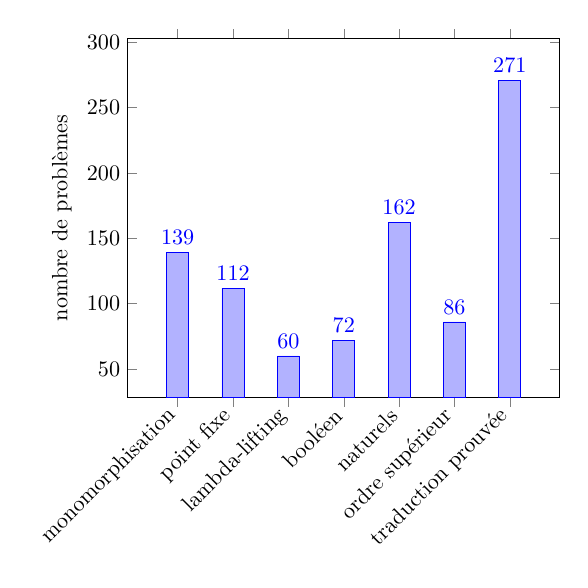
\begin{tikzpicture}[scale=0.8]
\begin{axis}[ybar,enlargelimits=0.15,legend style={at={(2,2)},anchor=north,legend columns=0},ylabel={nombre de problèmes},symbolic x coords={monomorphisation,point fixe,lambda-lifting,booléen,naturels,ordre supérieur,traduction prouvée},xtick=data,
nodes near coords,
nodes near coords align={vertical},
x tick label style={rotate=45,anchor=east},]
\addplot coordinates {(monomorphisation,139) (point fixe,112) (lambda-lifting,60) (booléen,72)(naturels,162)(ordre supérieur,86)(traduction prouvée,271)};
\end{axis}
\end{tikzpicture}


<<<<<<< HEAD
\subsection{Efficacité de \beagle}
A travers ses exemples, il est difficile de juger de la qualité de \beagle
face à \metis puisque \metis résout l'ensemble de ses buts rapidement.
Parmi les problèmes, nous avons retenu 69 problèmes contenant au moins un théorème donné par l'utilisateur contenant uniquement des constantes arithmétiques $+$,$-$,$\leq$,$<$,$\geq$,$>$ et nous avons supprimés 79 tels théorèmes. \metis n'est donc plus en mesure de résoudre l'un de ses problèmes modifiés. Cependant \beagletac y parvient:


\noindent \begin{tabularx}{\textwidth}{|X|X|}
\hline
Résultats & Utilisation du code \\
\hline
\begin{tikzpicture}[scale=1.5,baseline=(current bounding box.center)]
    \slice{0/100*360}
          {88/100*360}
          {88\%}{insatisfaisable}{green}
    \slice{88/100*360}
          {97/100*360}
          {9\%}{inconnu}{red}
    \slice{97/100*360}
          {100/100*360}
          {3\%}{time out}{red}
\end{tikzpicture}
&
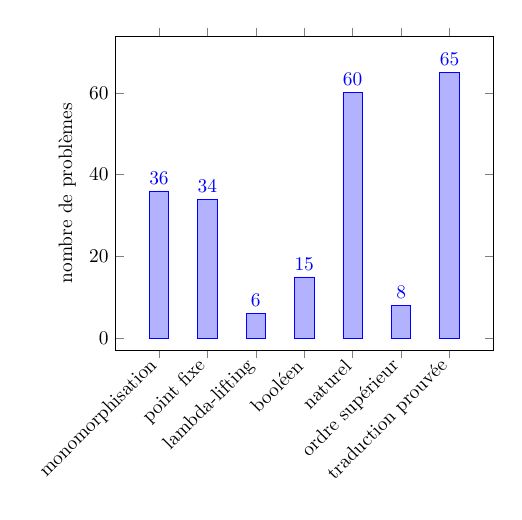
\begin{tikzpicture}[scale=0.7,baseline=(current bounding box.center)]
\begin{axis}[ybar,enlargelimits=0.15,legend style={at={(2,2)},anchor=north,legend columns=0},ylabel={nombre de problèmes},symbolic x coords={monomorphisation,
point fixe,lambda-lifting,booléen,naturel,ordre supérieur,traduction prouvée},xtick=data,
nodes near coords,
nodes near coords align={vertical},
x tick label style={rotate=45,anchor=east}]
\addplot coordinates {(monomorphisation,36) (point fixe,34) (lambda-lifting,6) (booléen,15)(naturel,60)(ordre supérieur,8)(traduction prouvée,65)};
\end{axis}
\end{tikzpicture}
\\
\hline
\end{tabularx}


\subsubsection{Expressivité}

Grâce à notre traduction, \beagletac permet de résoudre des problèmes
combinant d'ordre supérieur avec arithmétique, lorsque le raisonnement
propositionnel est du premier ordre. Cette tactique est donc plus
expressive que \metistac, puisqu'il n'est pas besoin de fournir les
lemmes arithmétiques utilisés.


